\documentclass[a4paper,10pt]{article}
\usepackage{a4wide}
\usepackage{listings}
\usepackage{mathtools}
\usepackage[english]{babel}
\usepackage{graphicx}
\begin{document}
\section*{Authors, date, assignment}
Authors : Dan Iatco (s2535130) \& Levente Sandor (s2552310)\\
Group: CS 1.Ib.1\\
Date:  13 December 2013\\
Day, Time of the Lab session: Thursday 28 November 2013, 15:00-17:00\\
Autonomous Systems lab 3 "Genetic Algorithms"\\

\section*{Exercise 1}
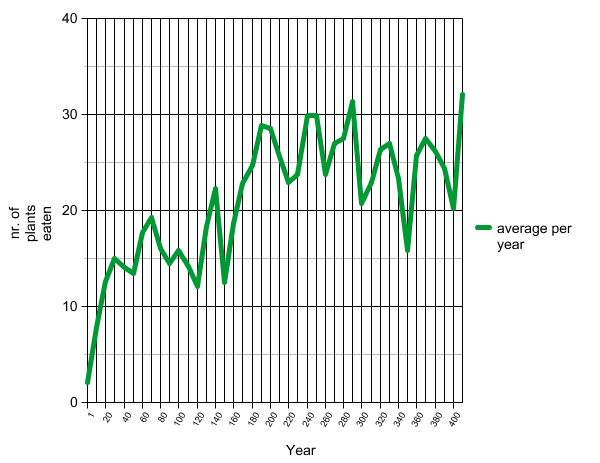
\includegraphics[width=10cm]{graph5.png}\\
From graph 1 we can easily observe that the eaters' fitness oscillates rather dramatically, but the average fitness increases (up to a point). From the second graph we can observe how fast the eaters are evolving and the graph is not monotonic either, which means that there is a chance that the next generation will be genetically inferior to the previous one. To determine to which value the average amount of plants eaten converge we let the simulation run 5 times up to the year 400 with the default settings. 
The results were:\\[0.2cm]
1st run: 26.7478\\
2nd run: 27.8144\\
3rd run: 26.7286\\
4th run: 25.5803\\
5th run: 23.7150\\[0.2cm]
We can conclude from this data that the average amounts of plants eaten converges
to around 26,11.

\section*{Exercise 2}
Eaters are primitive organisms which have a genetic code, DNA. At the start of their existance in the simulated world,
their DNA contain very few information about the world. They do not have any experience, and their movement is chaotic,
one cannot observe a low for their trajectory. As the time pass, the eaters evolve, and after 100 one can already observe
regularity in their movement, and also the numbers of plants eaten raised.\\ In conclusion the eaters adapted to sorvive
in the simulated world.

\section*{Exercise 3}
\includegraphics[width=10cm]{graph_ex3.png}\\
At 0\% mutation probability, the average score at 400 years is highly random, but very stable, since the genetic makeup of the later generations stays very close to the initial one. With 0.25\% chance of mutation, we get very stable and fast progress, it being apparently the ideal value for the eaters. At 10\% we are likely to see a very low and unstable average fitness of the eaters.

\section*{Exercise 4}
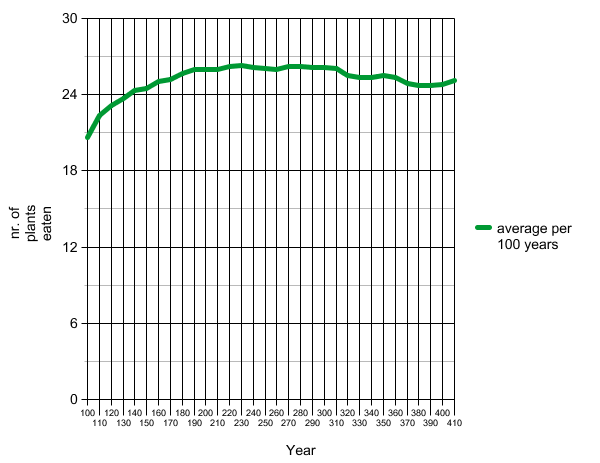
\includegraphics[width=10cm]{graph.png}\\
Crossover probability plays an important role in evolution, from the simulations we notice a difference between
between evolutions. The lower is the crossover probability, the worse an eater is evolving. This we can see on
the second graph, which represents the average plants eaten by an eater in 5 one hudred years average.\\
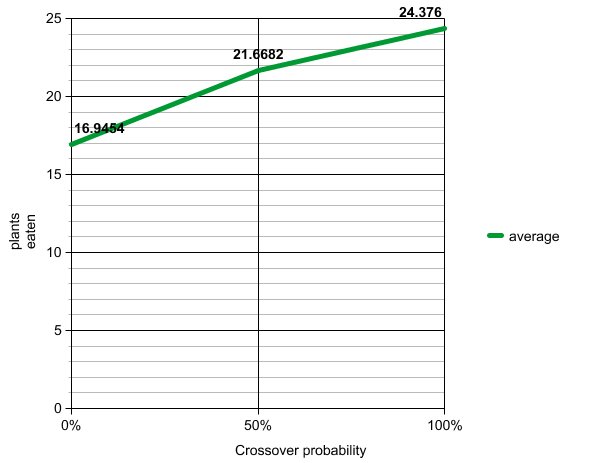
\includegraphics[width=10cm]{graph4.png}\\

\section*{Exercise 5}
To explore the world options, we used a 0.25\% chance of mutation, and made our observations after 100 years, ensuring the eaters adapt to their environment as best as they can.\\
If the plants grow in rows, eaters move horizontally, eating them, but as soon as they cannot find anymore, they start moving vertically until they find a new row of plants, which they start eating again. Their average score is also higher than that with the original settings.\\
If plants grow in clumps, eaters will move in random directions until they hit a clump, in which case they start systematically consuming them. Their average score is marginally higher than with the original settings.\\
If plants grow at random, they cannot develop a way to find them, so their search becomes very inefficient and their average score stays low.\\
If plants grow at the bottom or along the edges, a good portion of eaters will always stay near them, eating at a constant rate, while others just move randomly. This usually leads to a really high average score, but huge gaps between the scores of the eaters themselves.\\
Unsurprisingly, the approximate population of eaters has little effect on the average score. The location of new plants has a great influence though - eaters behave completely differrently if the plants regrow nearby - they will usually stick around and circle after eating one, instead of moving in straight lines.\\
It is ideal for eaters to be born at their parents' location - more successful eaters will have more successful children this way. Starting in different positions can be benefitial or detrimental to the population's success depending on plant settings.

\end{document}
